\section{Creation of DeepFakes}\label{sect:creation-of-deepfakes}
Statistical models come in multiple classes with divergent properties.
Two of such classes are discriminative and generative models. Generative models
learn the statistical properties of their input domain~\cite[cf.][\nopp{}651\psqq]{Goodfellow.2016}.
For example, they are able to generate unique images of human faces, based on
previously observed ones~\cite{Karras.2019}.

\par
Generative models are thus the focus of techniques for creating \textit{DeepFakes}. As
this serves as an introduction to the creation of \textit{DeepFakes}, we limit the scope
to:
% Description of basic network types
\begin{description}[leftmargin=0cm]
    \item[\glspl{ed}] \glspl{ed} consist of at least two networks, \gls{en} and
    \gls{de}. The \gls{en}-part is trained to extract
    useful features \(\text{En}(x)=e\) from input image \(x\). This is often
    done by narrowing layer-width towards its center (see \cref{subfig:ed}) or
    some other regularization criterion~\cite[cf.][499-505]{Goodfellow.2016}.
    After encoding \(x \rightarrow e\), \(e\) is fed into \gls{de} to arrive at
    the final result \(\text{De}(e)=x_g\). \Glspl{ae} are a special form of
    \gls{ed}, where the network is trained to reproduce its inputs, i.e.\
    \(\text{De}(\text{En}(x))\approx x\).

    \item[\glspl{gan}] \glspl{gan}, like \gls{ed}, consist of at least two networks,
    \gls{gen} and \gls{disc} (see \cref{subfig:gan}). In a sense, \gls{gen} can
    be interpreted similar to the \gls{de} part of the \gls{ed}. But, instead of
    relying on \gls{en} to extract features \(\text{En}(x)=e\), the input
    \(z\) is sampled from a so called prior-distribution \(z\sim p_z\), e.g.\
    the normal distribution \(p_z=\mathcal{N}(0, 1)\). Then, using \(z\),
    \gls{gen} generates images \(\text{G}(z)=x_g\). \Gls{disc}, on the other hand,
    tries to discern whether an input is from the identity of the target
    \(x\in X_{\text{target-id}}\) or artifically generated by \gls{gen}, i.e.\ \(x_g\).
    \Gls{gen} and \gls{disc} are then trained in alternation, such that \gls{gen}
    tries to fool \gls{disc} into \textit{thinking} that \(x_g\) is an image from the
    target \(X_{\text{target-id}}\) and \gls{disc} trying to discern correctly
    between \(x\sim X\) and \(x_g\sim \text{G}(p_z)\). That way, we are able to
    generate realistically looking faces similar to that of the target~\cite{Goodfellow.2014}.
\end{description}
% Figure of basic network types
\begin{figure}[h]
    \centering
    \subcaptionbox{\label{subfig:ed}}{
        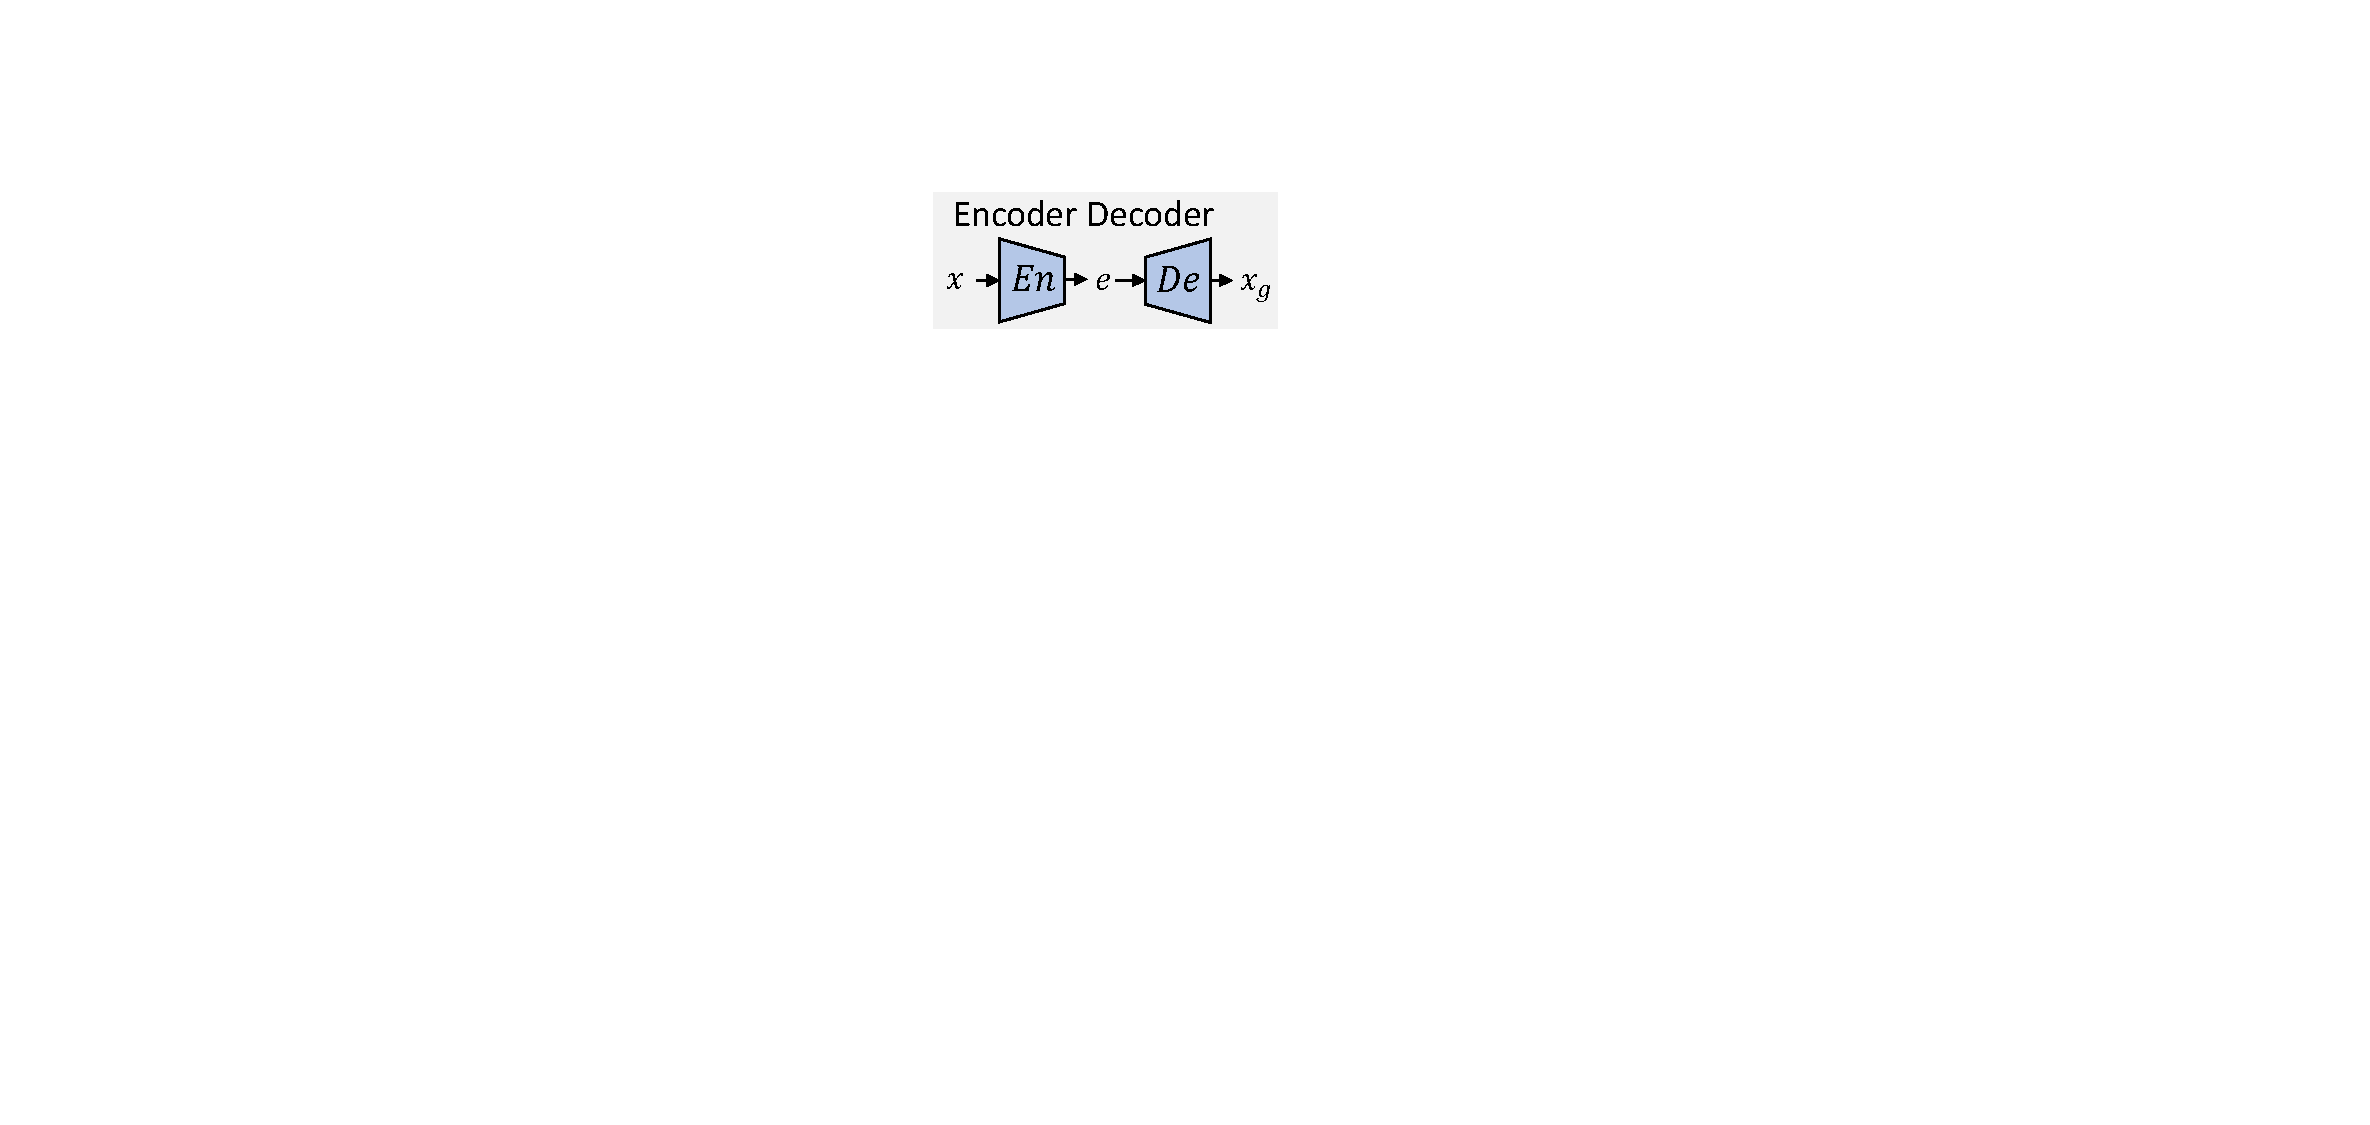
\includegraphics[width=3.3cm]{nns_ed.pdf}
    }
    \subcaptionbox{\label{subfig:gan}}{
        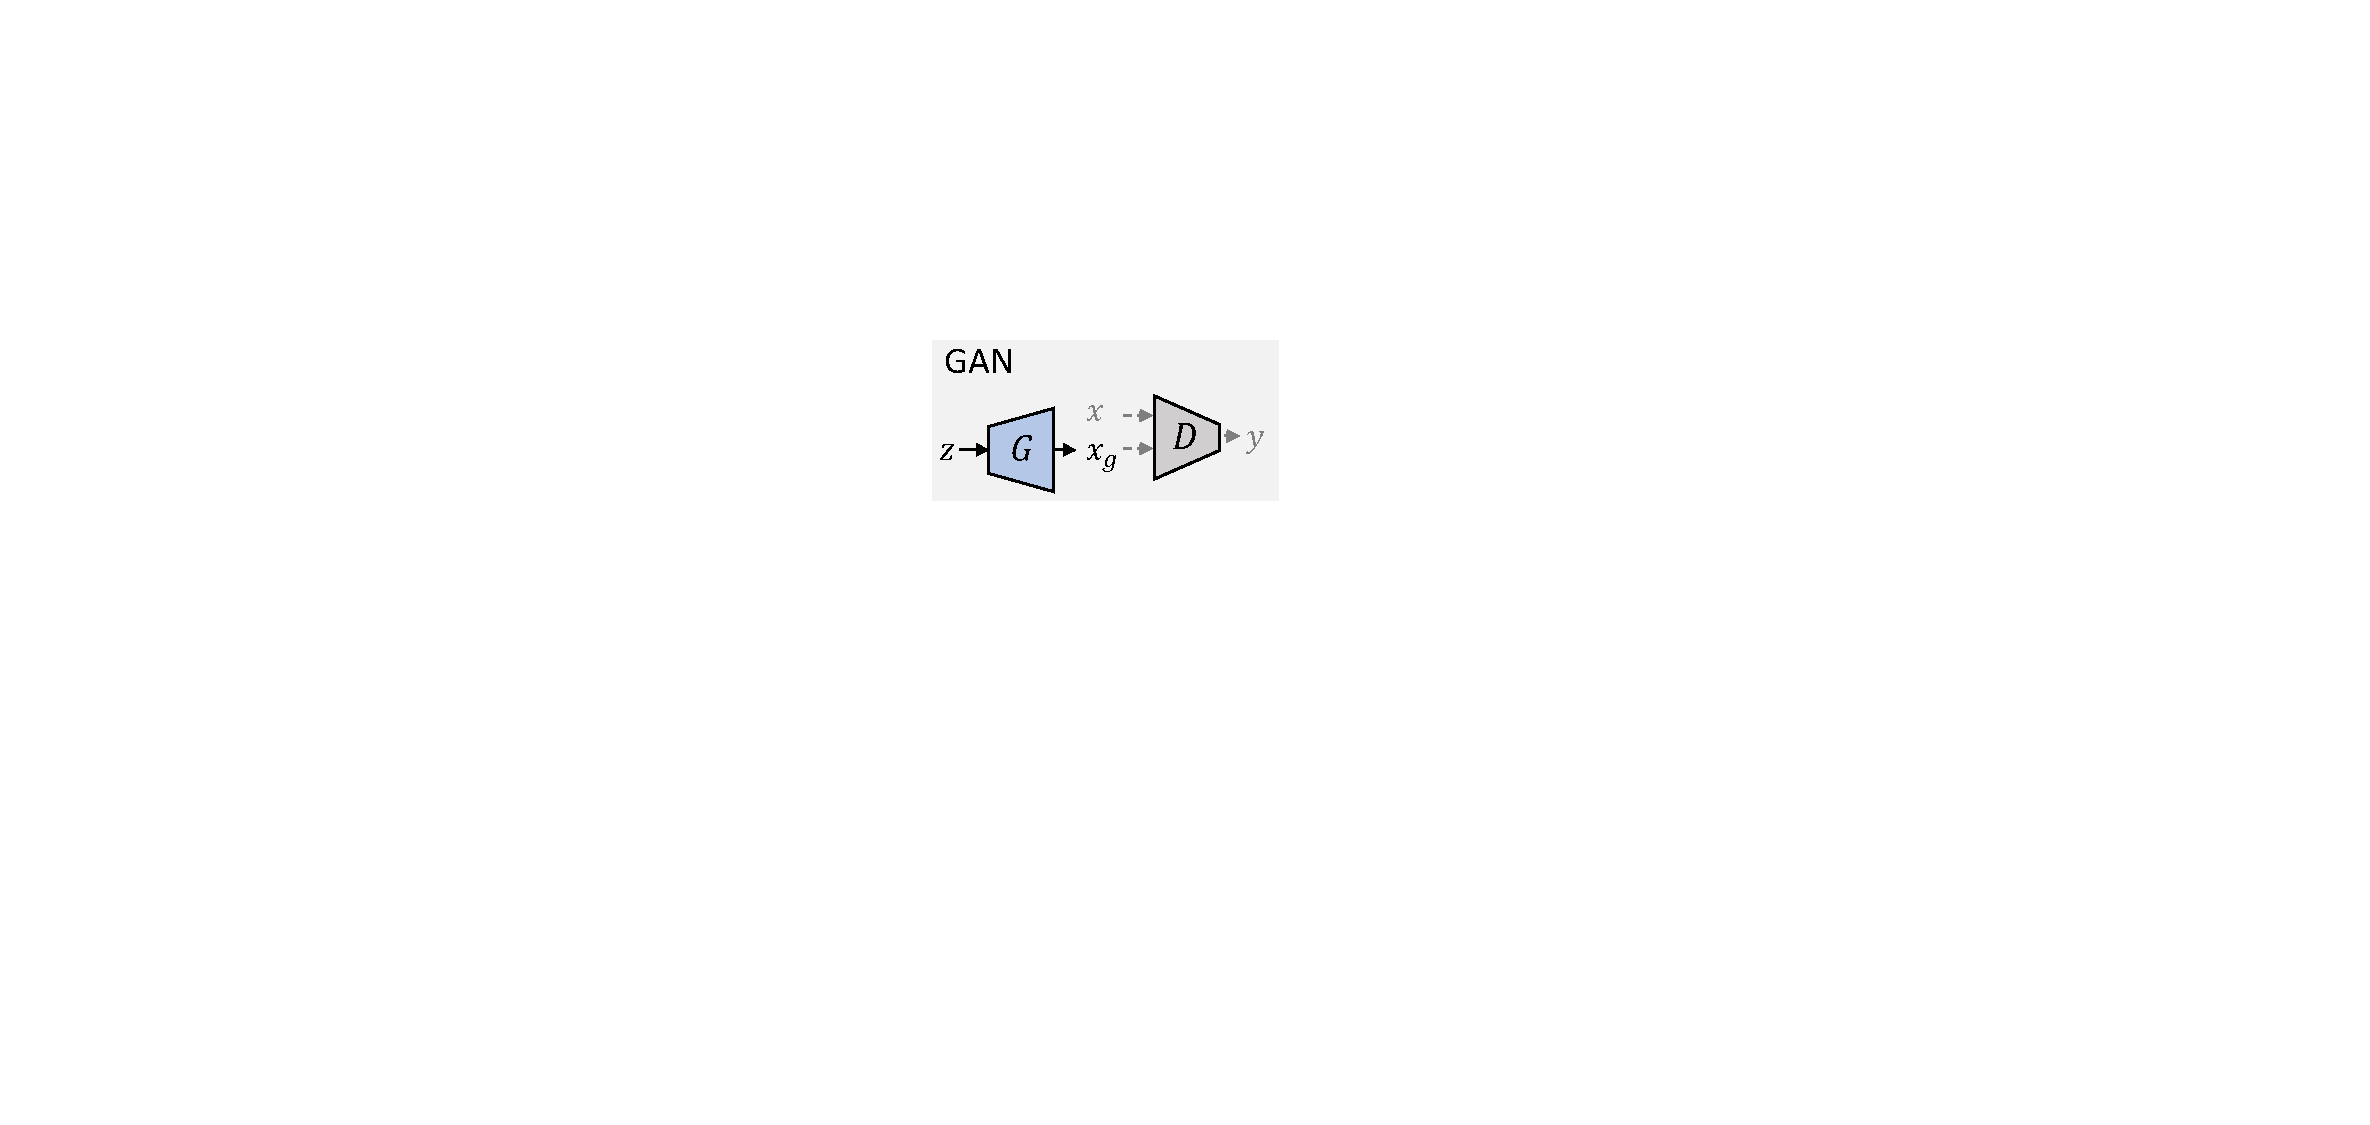
\includegraphics[width=3cm]{nns_gan.pdf}
    }
    \subcaptionbox{}{
        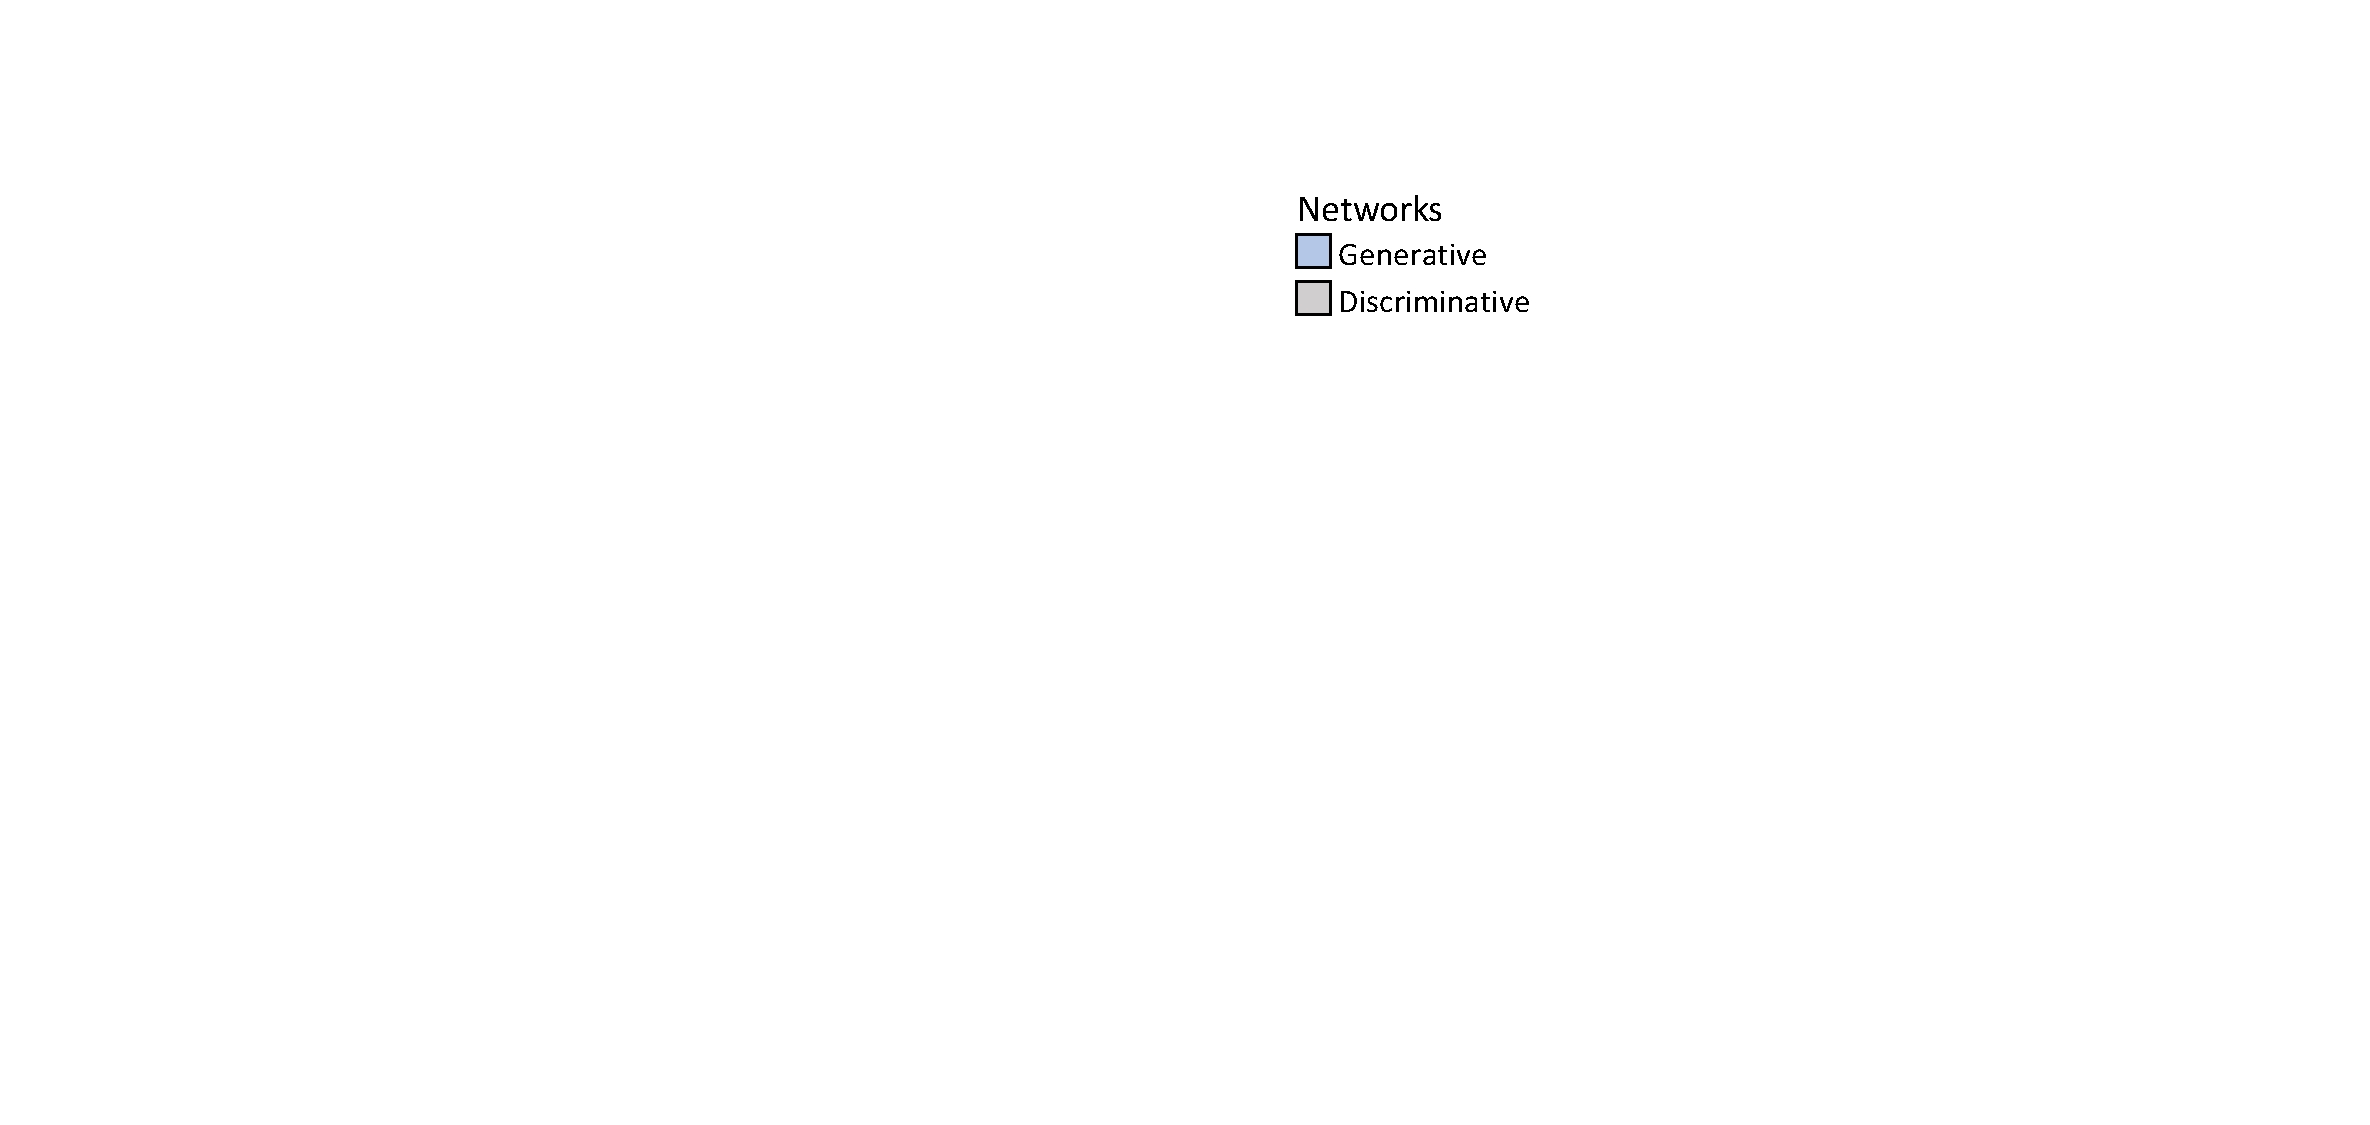
\includegraphics[width=2.5cm]{nns_description.pdf}
    }
    \caption{Selection of generative models, adopted from~\cite{Mirsky.2020}}\label{fig:generative-models}
\end{figure}

When trying to create believable face reenactment footage, there are three \textbf{goals}
we try to reach in the final generated image \(x_g\):
\begin{enumerate}[1.)]
    \item to preserve the mimic of driver \(x_d\) in \(x_g\), s.t.\ \(\text{mimic}(x_d)=\text{mimic}(x_g)\)\label{goal:mimic-perservation}
    \item to preserve the identity target \(x_t\) in \(x_g\), s.t.\ \(\text{id}(x_t)=\text{id}(x_g)\)\label{goal:preserve-identity}
    \item to generate a realistically looking image\label{goal:increase-realism}
\end{enumerate}
We can take these goals and construct a model after them. In order to generate
an image we utilize the \gls{ed}-model from \cref{subfig:ed}

\subsection{Preserving Mimic}
To tackle goal~\ref{goal:mimic-perservation}, one must define how to
numerically represent the mimic of a face, \(\text{mimic}(x)=\textit{undefined}\).
Two such representations are
\begin{enumerate*}[a.)]
    \item via facial landmarks or
    \item via the \gls{facs}
\end{enumerate*}
For simplicity, only \gls{facs} is considered. A discussion of facial landmarks
can be found in e.g.\ \cite{Ha.2020}.

\paragraph*{Facial Action Coding System (FACS)}
The \gls{facs} was introduced in 1978 by \textcite{Ekman.1978}. They grouped
muscle regions of the face to 58 so called \glspl{au}, which can be represented
by vectors. A major advantage of \glspl{au} over facial landmarks is that they
are (more or less) invariant (i.e.\ the same expression is encoded similarly)
between faces, head angle and scale~\cite{Pham.2018}.

\par
Following this discussion, \gls{facs} is used. \Glspl{au} might be computed using
a generic \gls{aue}, e.g.\ \cite{Senechal.2015}. The \gls{au}-vectors are then
concatenated to the encoded representation (\(\text{En}(x_t)=e\)) and used in
the \gls{de}-step. To enforce goal~\ref{goal:mimic-perservation}, the difference
in \glspl{au} between final \textit{DeepFake} \(\text{AUE}(x_g)=a_g\) and driver
\(\text{AUE}(x_d)=a_d\) are minimized in training: \(\min{(\left|a_g-a_d\right|)}\).
A visualization of this is given in \cref{fig:gath-aue}.
\begin{figure}[htp]
    \center{}
    \vspace{-.5em}
    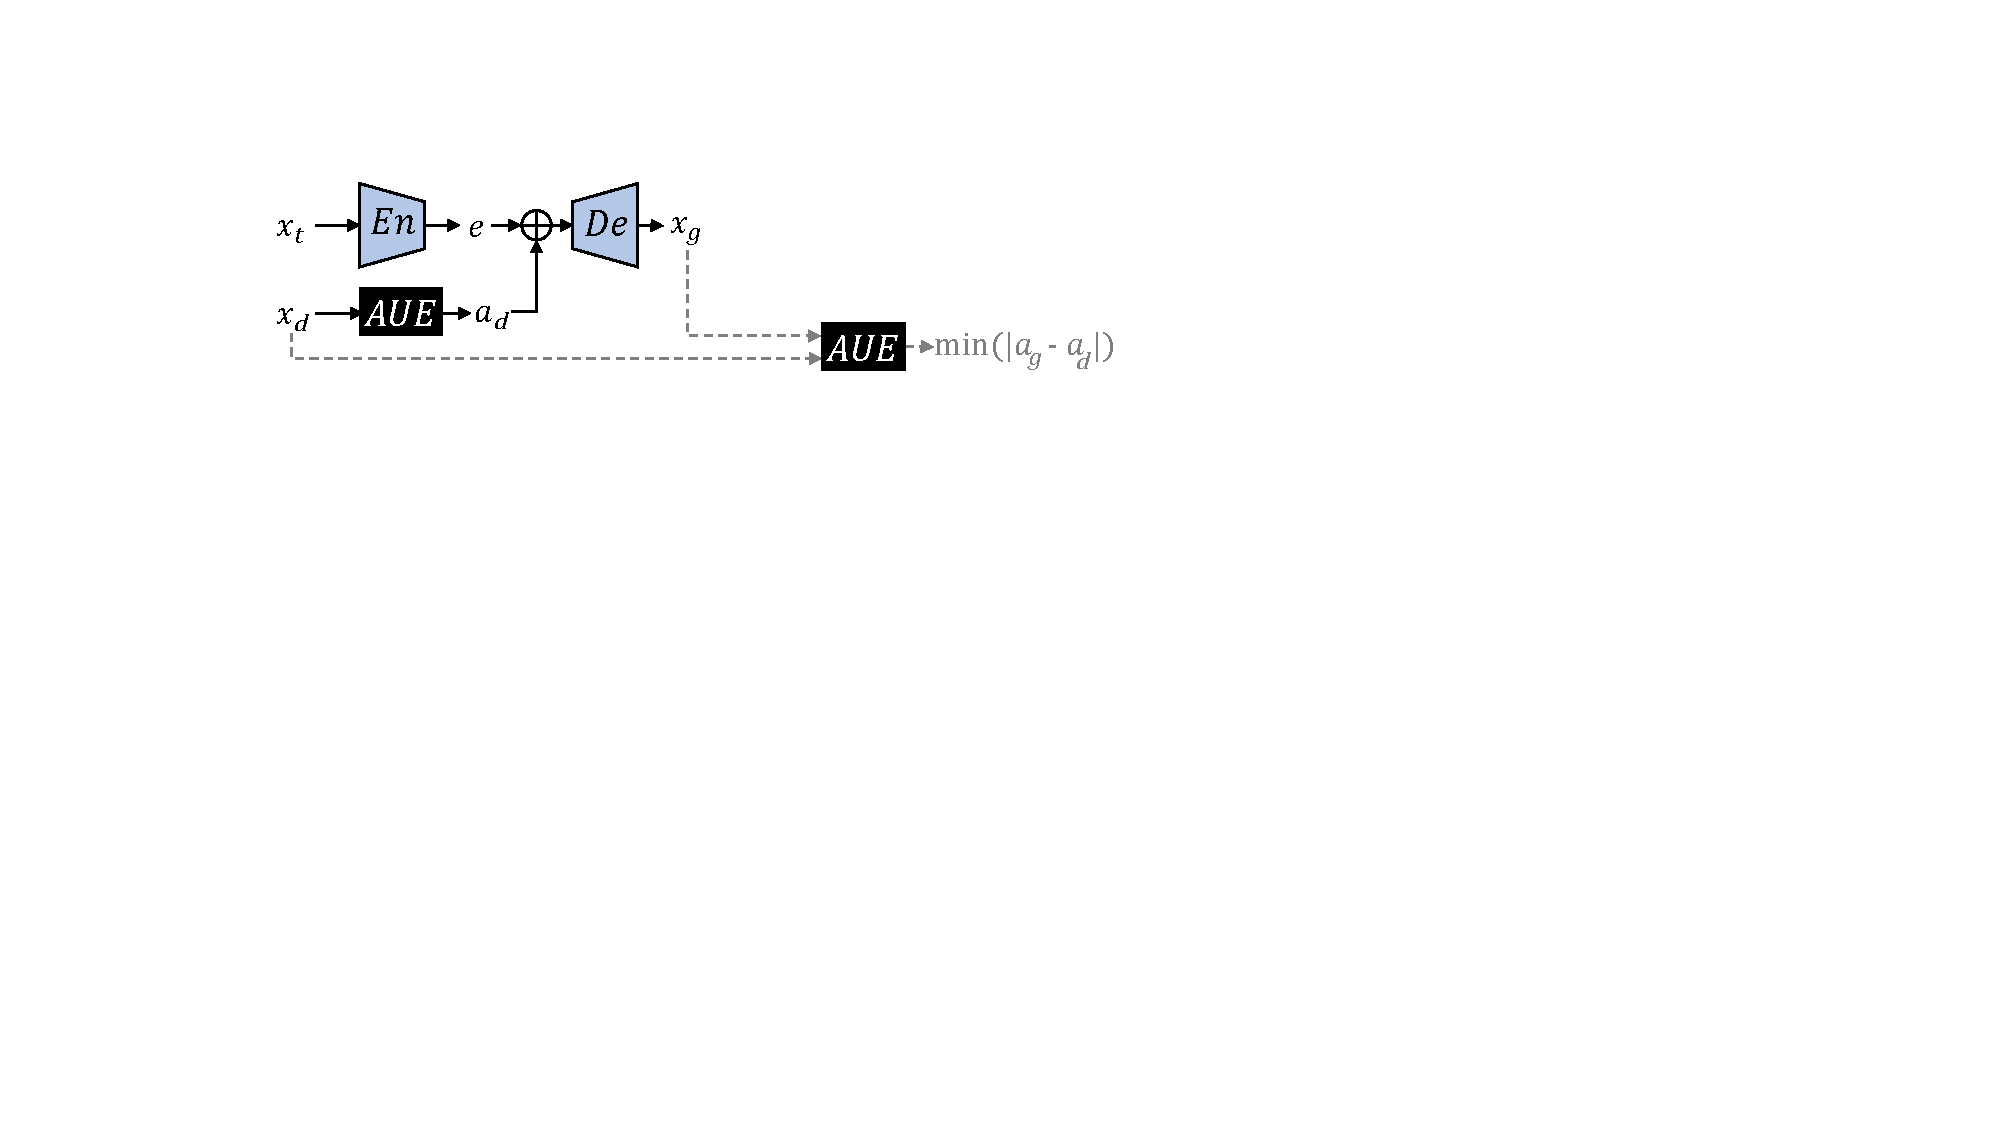
\includegraphics[width=.57\textwidth]{gath_aue.pdf}
    \caption{\gls{ed}-architecture enriched with \glspl{au}, where \(\bigoplus\)
    denotes concatenation. Grey paths are used solely in training. Inspired
    by~\cite{Mirsky.2020, Pham.2018}}\label{fig:gath-aue}
    \vspace{-2em}
\end{figure}

\subsection{Preserving Identity}
Training the model on preserving the identity of the target requires a training
set of known targets, e.g.\ \cite{Chen.2015,Cao.2014,Tarres.2011} which together
consist of about 2000 identities~\cite{Pham.2018}. One can then learn an image
classifier \(I\), e.g.\ MobileNet~\cite{Howard.2017} (for its simplicity and speed)
to assign the correct identity to a given image. Once the classifier \(I\)
converges, it can be added to the training procedure of the model. The \gls{ed}
model can then be trained to also minimize the cross-entropy identity loss
\(\mathcal{L}_{id}\) (see \cref{eq:identity-loss}). A visualization of this is
given in \cref{fig:gath-aue-id}.
\begin{figure}[htp]
    \vspace{-.5em}
    \center{}
    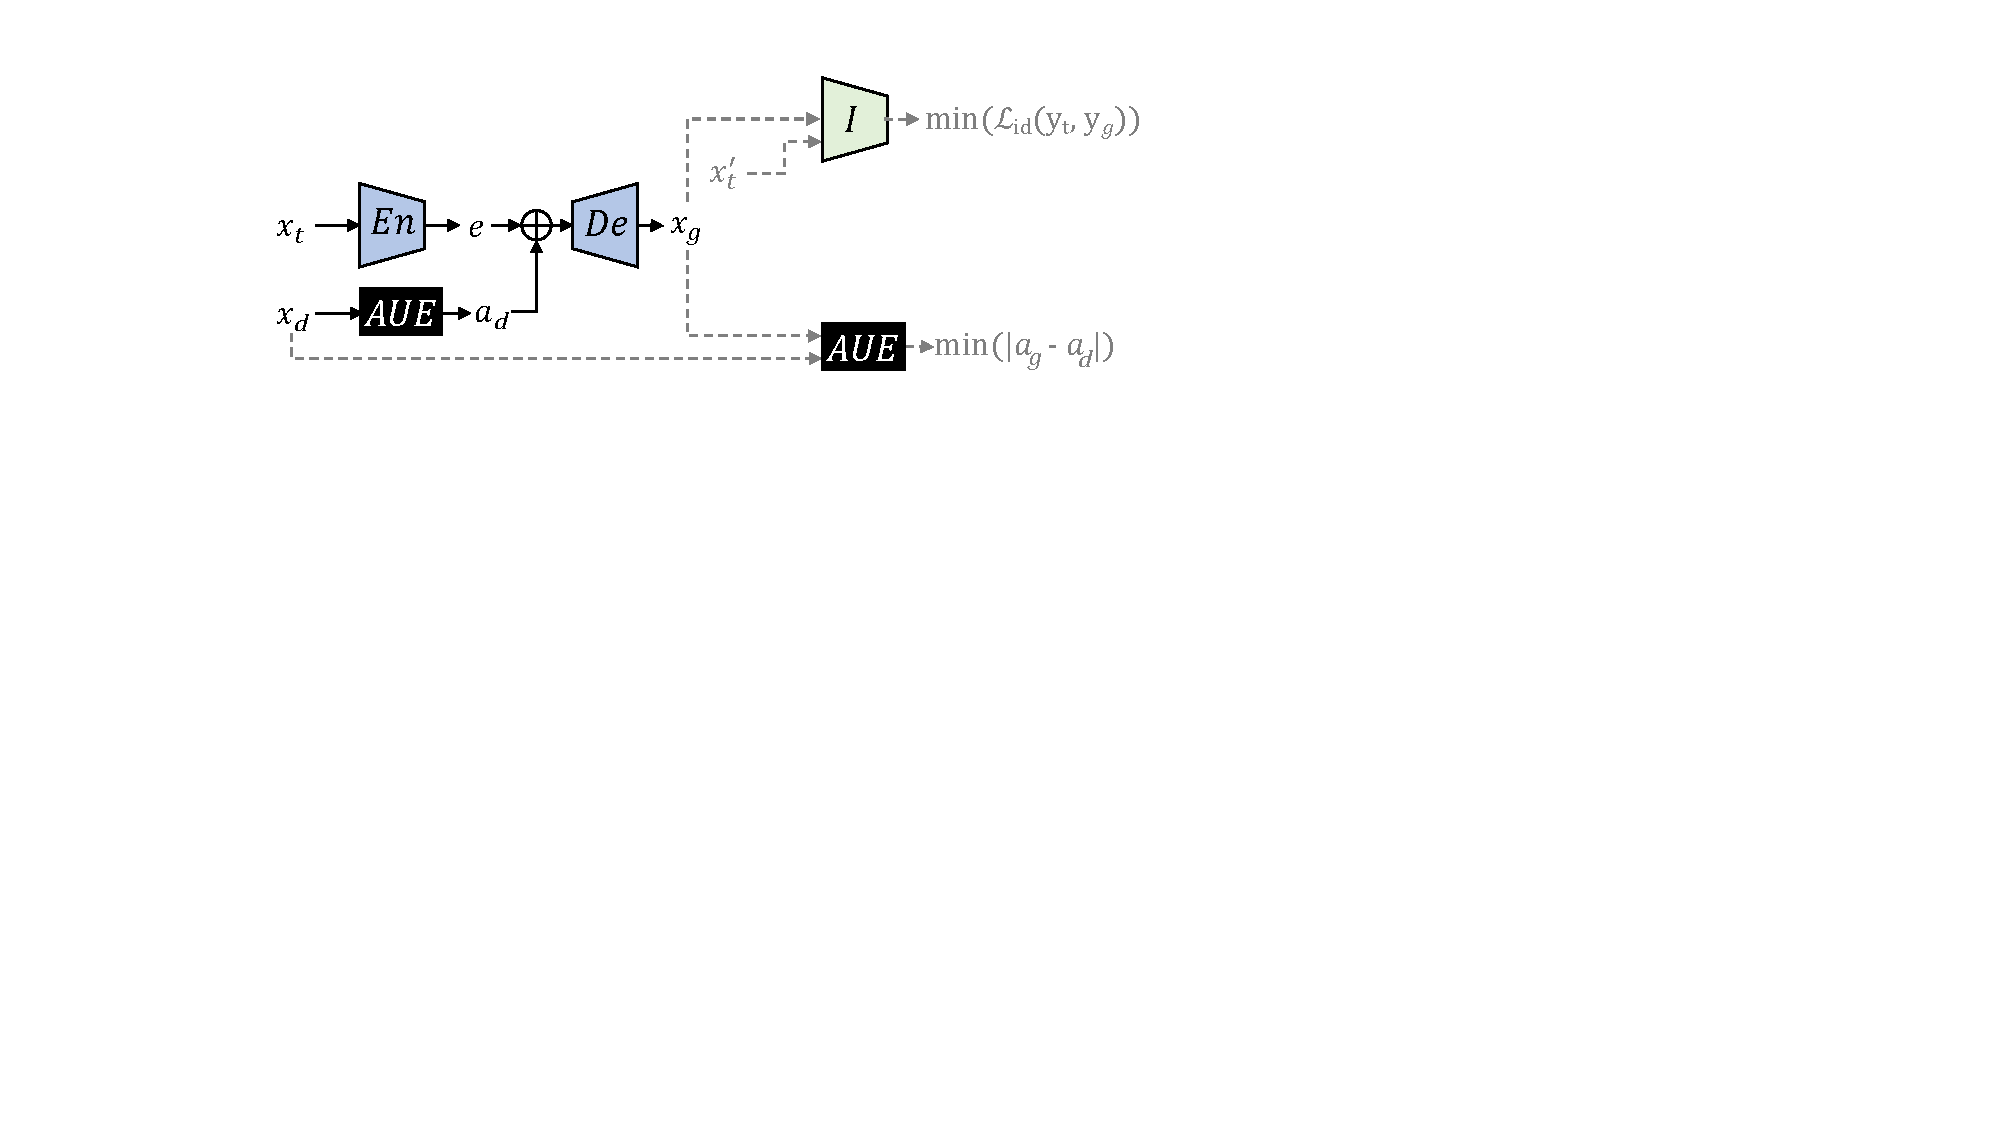
\includegraphics[width=.59\textwidth]{gath_aue_id.pdf}
    \caption{Architecture from \cref{fig:gath-aue}, enriched with an identity
    constraint, where \(x'_t\) is a randomly chosen image with identity of the target
    \(t\). Inspired by~\cite{Mirsky.2020, Pham.2018}}\label{fig:gath-aue-id}
    \vspace{-2em}
\end{figure}

\subsection{Increasing Realism}
Finally, to increase realism (goal~\ref{goal:increase-realism}), a \gls{gan}-inspired
discriminator \gls{disc} (see \cref{subfig:gan}) is adopted and trained alternatingly
to discern between real and generated images, minimizing the adversarial loss
\(\mathcal{L}_{adv}\)  (see \cref{eq:adversarial-loss}). A visualization of this
is given in \cref{fig:gath-aue-id-disc}.
\begin{figure}[htp]
    \vspace{-1em}
    \center{}
    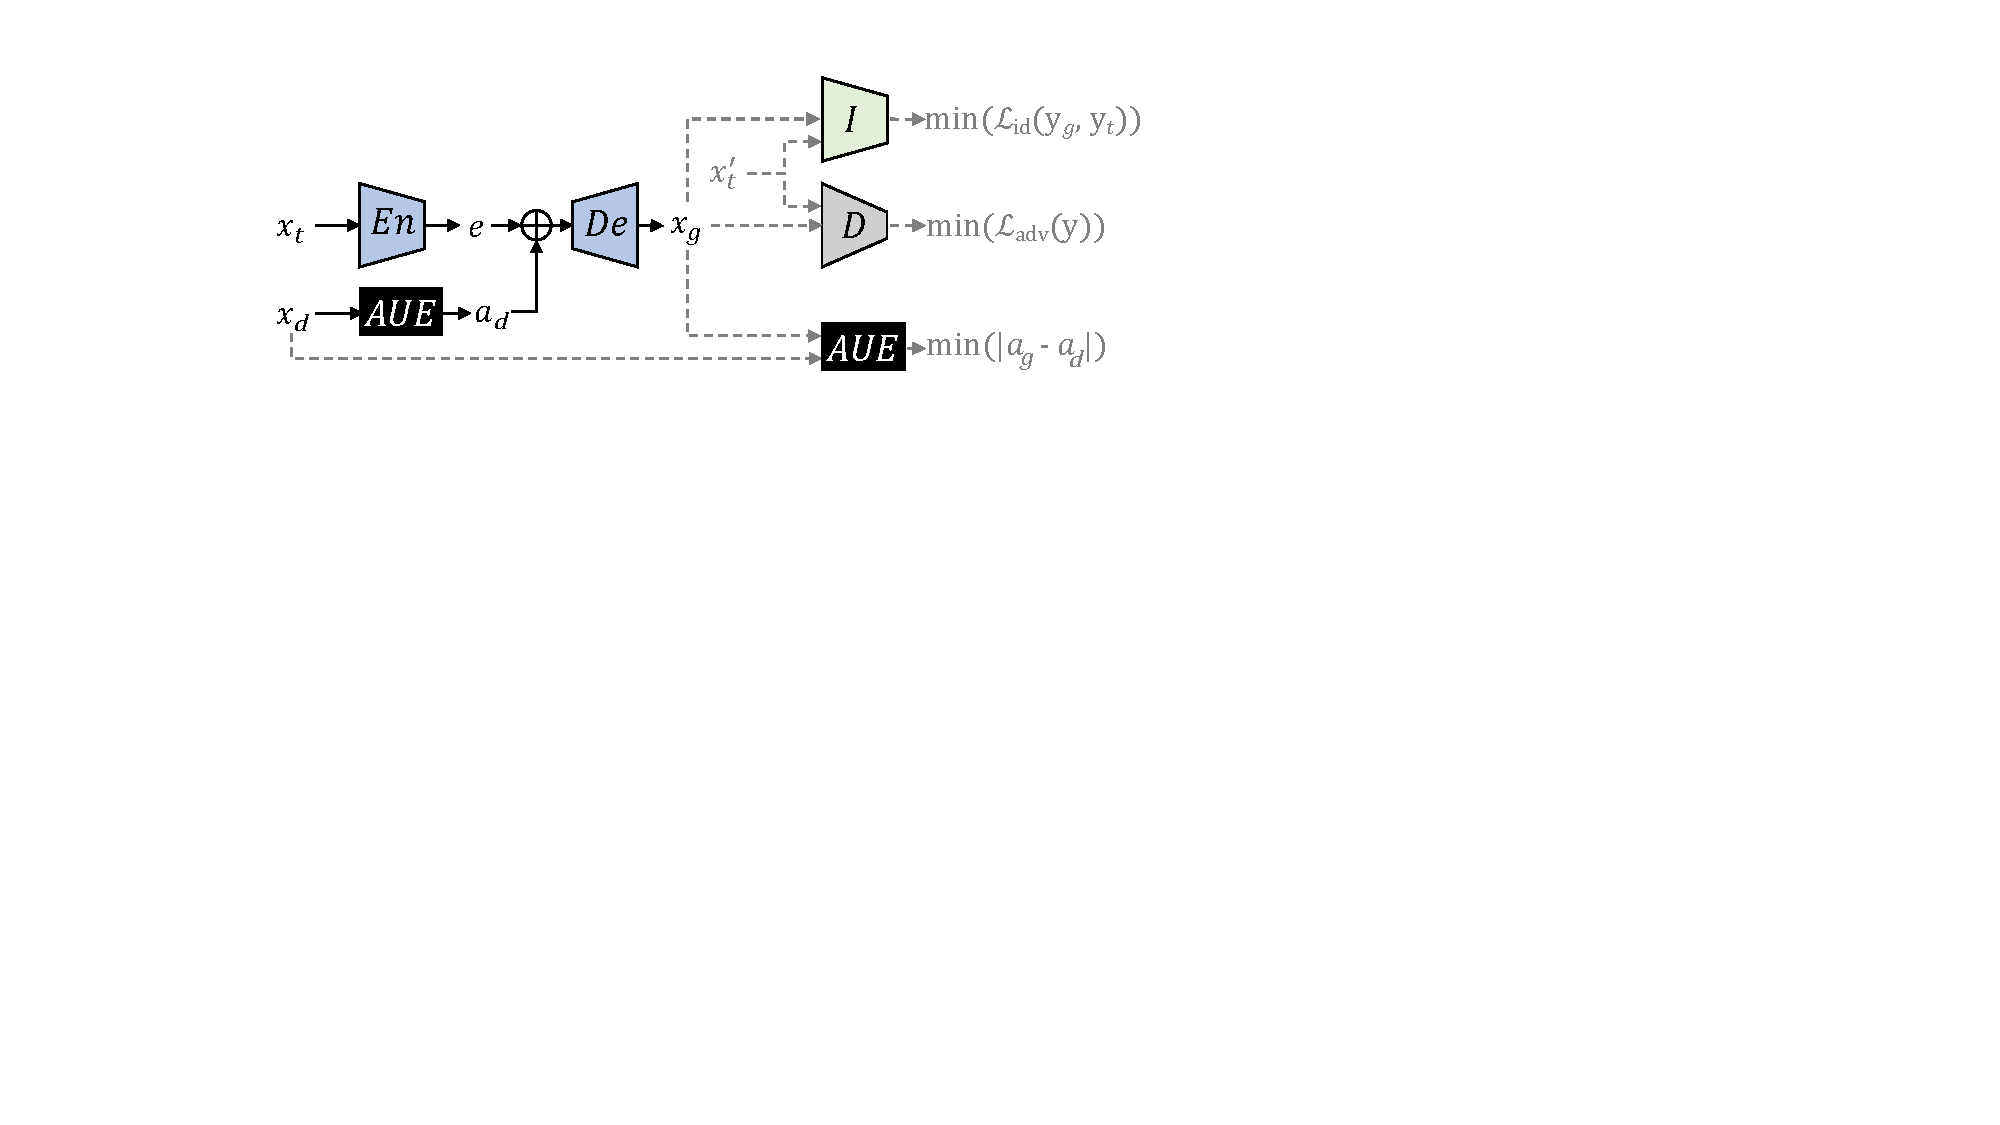
\includegraphics[width=.59\textwidth]{gath_aue_id_disc.pdf}
    \caption{Architecture from \cref{fig:gath-aue-id}, enriched with a realism
    constraint. Inspired by~\cite{Mirsky.2020, Pham.2018}}\label{fig:gath-aue-id-disc}
    \vspace{-3em}
\end{figure}